\graphicspath{{./img/}}

\subsection{C vs ASM}

{\scshape\Large solver$\_$set$\_$bnd\par}

Como se puede apreciar en las figuras de la sección anterior, ASM tiene clocks mucho menores a las funciones en C en todos los tamaños si bien en los mas chicos (por ejemplo 16) las performances entre C y ASM son bastante equivalentes, como lo demuestra el gráfico de abajo. A su vez también vemos que la matriz U tarda en procesar mas ciclos de clock que la matriz V.

\begin{figure}[h]
  \centering
  	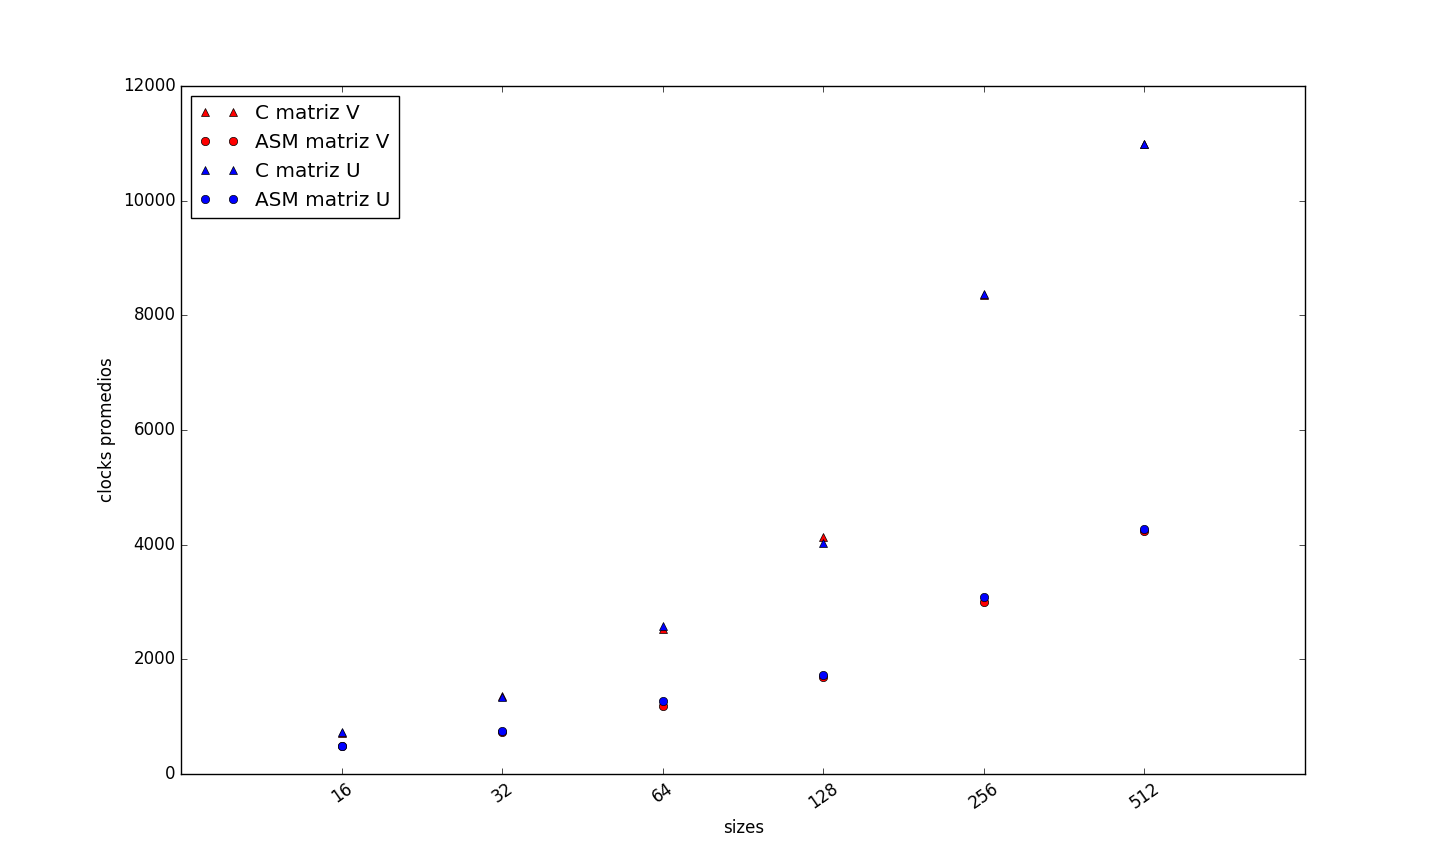
\includegraphics[width=.6\linewidth]{ClocksCYASM.png}
  	\caption{ASM VS C solver$\_$set$\_$bnd}
  	\label{fig:ASMU}
\end{figure}

A su vez, si en vez de 750 repeticiones se hicieran menos, los datos que se obtienen cada vez son mas proclives a errores. Concluimos que por la ley de los grandes números cuando tenemos una muestra menor se pueden producir varios errores en las experimentaciones como lo demuestra el siguiente gráfico con 200 iteraciones. Se pueden comparar fácilmente con los datos obtenidos y postulados en la sección Resultados.

\begin{figure}[h]
  \centering
  	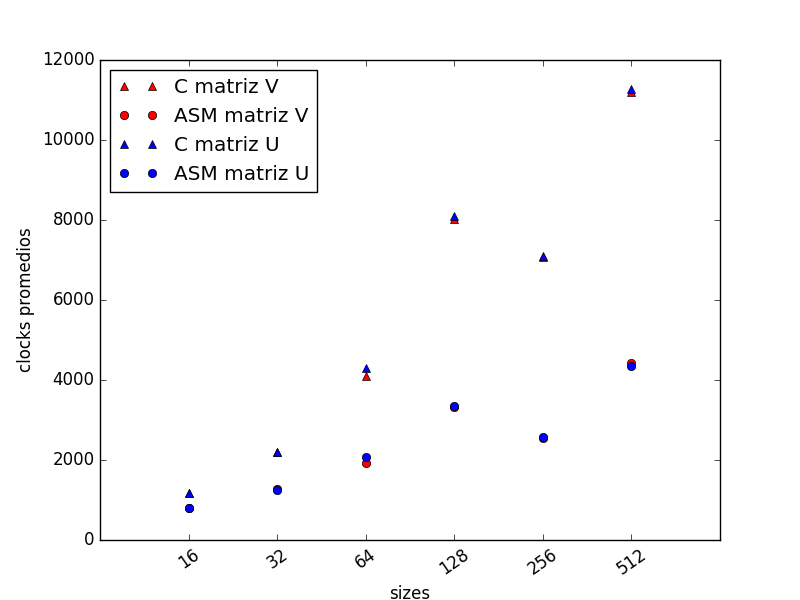
\includegraphics[width=.6\linewidth]{ClocksCYASMMAL.png}
  	\caption{ASM VS C solver$\_$set$\_$bnd con 200 iteraciones}
  	\label{fig:ASMU}
\end{figure}

{\scshape\Large solver$\_$lin$\_$solve\par}

Se puede ver que asm tarda menos que todos los niveles de optimizacion para los tres tamaño de matrices. Para poder tener mas certeza que esto pasa y de que los outliers no sean muchos en cada muestra, en vez de probar con 1000 repeticiones el experimento anterior, se probo con 50, 125, 250, 500, 2000 y 3000. Y se puede observar que los nuevos graficos son muy similares a los del experimento de la seccion resutados. Entonces esto no quiere decir que asm tarda menos que los diferentes niveles de optimizacion tanto para pocas repeticiones como muchas. 

\begin{figure}[h]
  \centering
  	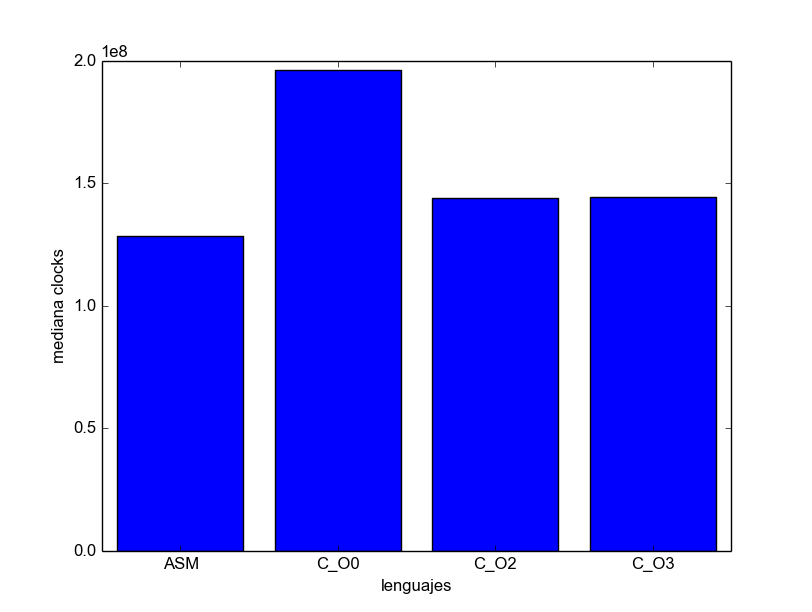
\includegraphics[width=.6\linewidth]{Matriz_512_50.png}
  	\caption{Performance para matriz de 512x512 con 50 repeticiones}
  	\label{fig:M50it}
\end{figure}

\begin{figure}[h]
  \centering
  	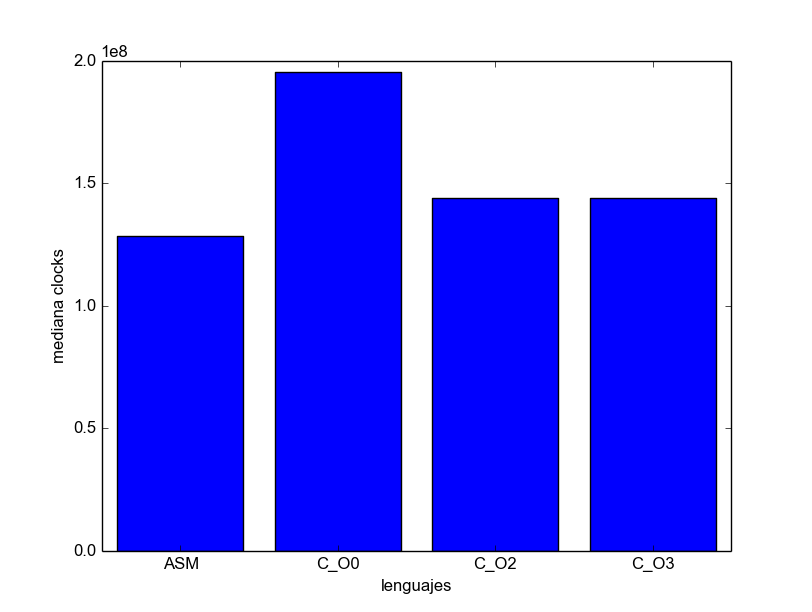
\includegraphics[width=.6\linewidth]{Matriz_512_500.png}
  	\caption{Performance para matriz de 512x512 con 500 repeticiones}
  	\label{fig:M500it}
\end{figure}

\begin{figure}[h]
  \centering
  	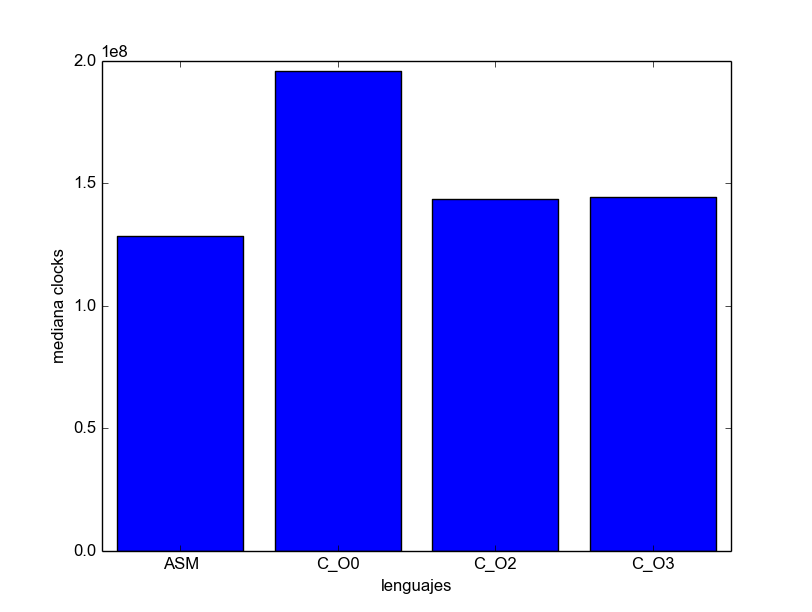
\includegraphics[width=.6\linewidth]{Matriz_512_3000.png}
  	\caption{Performance para matriz de 512x512 con 3000 repeticiones}
  	\label{fig:M3000it}
\end{figure}
